\chapter{Refactoring}

\section{Code-Smells} \label{sec:smells}

\subsubsection{Long-Class} 

\autoref{code:long-class-before} und \autoref{code:long-class-after} zeigen den Code eines Long-Class-Code-Smells 
vor (Commit \texttt{174283ab}) und nach (Commit \texttt{b0ce98af}) der Behebung mittels Aufteilen der Klasse 
in drei neue Klassen, die aber jeweils ein gemeinsames Interface (\textit{Parser}) implementieren. \\
Vorher gab es eine \textit{ArgumentParser}-Klasse, die als Methoden-Sammlung für das Parsen von 
\textit{CraftingPlan}s (\textit{parseConstructible}), \textit{Dice} (\textit{parseDice}) 
und \textit{Card}s (\textit{parseCards}) zuständig war. Hierdurch war die Klasse nicht SRP- oder OCP-konform 
und trug den Long-Class-Code-Smell. \\
Dies wurde in \autoref{code:long-class-after} gelöst, 
indem die ArgumentParser-Klasse aufgeteilt wurde in \textit{CardParser}, \textit{CraftingPlanParser} und \textit{DiceParser},
die jeweils das \textit{Parser}-Interface implementieren und somit nur die \textit{parse}-Methode haben. 
(Außerdem wurden die \textit{switch}-Statements gleich mit aufgelöst, aber dieser Code-Smell wird hier nicht betrachtet).
Dadurch wahrt die neue Lösung das SRP und OCP und es ist keine long-class mehr. 

\lstinputlisting[
	label=code:long-class-before,    % Label; genutzt für Referenzen auf dieses Code-Beispiel
	caption=Long-Class-Code-Smell der \textit{ArgumentParser}-Klasse zum Commit \texttt{174283ab}.,
	captionpos=b,               % Position, an der die Caption angezeigt wird t(op) oder b(ottom)
	style=EigenerJavaStyle,   % Eigener Style der vor dem Dokument festgelegt wurde
	firstline=1,                % Zeilennummer im Dokument welche als erste angezeigt wird
	lastline=100                 % Letzte Zeile welche ins LaTeX Dokument übernommen wird
]{Quellcode/long-class-before.java}


\lstinputlisting[
	label=code:long-class-after,    % Label; genutzt für Referenzen auf dieses Code-Beispiel
	caption=Long-Class-Code-Smell behoben durch Aufteilung der Klassen zum Commit \texttt{b0ce98af}.,
	captionpos=b,               % Position, an der die Caption angezeigt wird t(op) oder b(ottom)
	style=EigenerJavaStyle,   % Eigener Style der vor dem Dokument festgelegt wurde
	firstline=1,                % Zeilennummer im Dokument welche als erste angezeigt wird
	lastline=100                 % Letzte Zeile welche ins LaTeX Dokument übernommen wird
]{Quellcode/long-class-after.java}

\subsubsection{Switch-Statement} 

\autoref{code:switch-before} und \autoref{code:switch-after} zeigen den Code eines Switch-Statement-Code-Smells 
vor (Commit \texttt{dd2a39d2}) und nach (Commit \texttt{a0e99692}) der Behebung mittels Einführung einer 
Map, die das Zählen dynamisch übernimmt. \\ 
Vorher gab es nur die \textit{CardDeck}-Klasse, die mit der \textit{isValid}-Methode überprüft, 
ob die Karten-Konfiguration (also die Anzahl der verschiedenen Karten im Deck) zulässig ist. 
Das Zählen der Karten funktionierte über ein Switch-Statement, welches einen explizit für diesen 
Kartentyp vorgesehenen Zähler inkrementierte, wenn die Karte bei Iteration über die Sammlung von eben diesem Typ war.
Der Vergleich auf Validität erfolgte über eine Kaskade von verundeten Gleichheitstests mit den erwünschten Werten. 
Diese Methode war furchtbar unerweiterbar. \\
Die Lösung in \autoref{code:switch-after} funktioniert so: Es wurde das neue VO \textit{CardDeckConfiguration} 
eingeführt, welches eine immutable Map von Card -> Integer mappt und ermöglicht zu überprüfen, ob zwei 
CardDeckConfigurations wertetechnisch gleich sind (\textit{record}'s implizites \textit{equals}). Zur 
besseren Vergleichbarkeit hat CardDeckConfiguration die \textit{withoutZeroOccurrences}-Methode, um Karten, 
die null Mal vorkommen, zu entfernen. CardDeck hat nun das Attribut \textit{config}, welches die erwünschte 
CardDeckConfiguration beinhaltet. Der Switch in \textit{isValid} wurde nun ersetzt, indem durch einen 
Loop über das CardDeck die Anzahl an Karten eines Typs dynamisch über eine Map-Struktur gezählt werden (Kartentyp 
ist der Schlüssel) und dann schließlich die Ist- und Soll-Konfiguration über ein \textit{equals}-Aufruf verglichen 
werden. Hierdurch wurde der Switch-Code-Smell entfernt und CardDeck ist nun OCP-konform, da nichts an der Klasse 
(also der frühere Switch und die Zähler pro Kartentyp und deren Vergleich) geändert werden muss, wenn ein neuer 
Kartentyp hinzugefügt wird.   

\lstinputlisting[
	label=code:switch-before,    % Label; genutzt für Referenzen auf dieses Code-Beispiel
	caption=Switch-Statement-Code-Smell der \textit{CardDeck}-Klasse zum Commit \texttt{dd2a39d2}.,
	captionpos=b,               % Position, an der die Caption angezeigt wird t(op) oder b(ottom)
	style=EigenerJavaStyle,   % Eigener Style der vor dem Dokument festgelegt wurde
	firstline=1,                % Zeilennummer im Dokument welche als erste angezeigt wird
	lastline=100                 % Letzte Zeile welche ins LaTeX Dokument übernommen wird
]{Quellcode/switch-before.java}


\lstinputlisting[
	label=code:switch-after,    % Label; genutzt für Referenzen auf dieses Code-Beispiel
	caption=Switch-Statement-Code-Smell behoben durch neue \textit{DeckConfiguration}-Klasse und Map zum Zeitpunkt des Commit \texttt{a0e99692}.,
	captionpos=b,               % Position, an der die Caption angezeigt wird t(op) oder b(ottom)
	style=EigenerJavaStyle,   % Eigener Style der vor dem Dokument festgelegt wurde
	firstline=1,                % Zeilennummer im Dokument welche als erste angezeigt wird
	lastline=100                 % Letzte Zeile welche ins LaTeX Dokument übernommen wird
]{Quellcode/switch-after.java}

\section{2 Refactorings}

\subsubsection{Extract-Method}

\autoref{fig:extract-before} und \autoref{code:extract-method-before} zeigen die \textit{isValid}-Methode 
der \textit{CardDeck}-Klasse\footnote{Wie in \autoref{sec:smells}.}
\underline{vor} dem \textit{Extract-Method}-Refactoring und \autoref{fig:extract-after} und \autoref{code:extract-method-after} \underline{nach}
dem Refactoring durch \underline{Commit \texttt{cb55ad97}}. \\
Extract-Method wurde hier angewandt, um die Lesbarkeit der \textit{isValid}-Methode deutlich zu erhöhen, da für den 
ersten Teil nicht direkt klar war, was passiert, wodurch fast ein Code-Comment-Smell benötigt worden wäre, ohne Method-Extraction. 
Nun ist in der isValid-Methode klar, was im ersten Zeil (zählen der eigenen Karten) und im zweiten Teil (Vergleich mit der Soll-Konfiguration) 
passiert. Außerdem ist die neue extrahierte Methode \textit{countCardOccurrences} eine recht allgemeine Methode, die ggf. in Zukunft 
noch an anderer Stelle verwendet werden kann, um Code-Duplication zu verhindern. 

\lstinputlisting[
	label=code:extract-method-before,    % Label; genutzt für Referenzen auf dieses Code-Beispiel
	caption=\textit{isValid}-Methode \underline{vor} Method-Extraction (aus u.a. Commit \texttt{a0e99692}). Vgl. \autoref{code:switch-after}.,
	captionpos=b,               % Position, an der die Caption angezeigt wird t(op) oder b(ottom)
	style=EigenerJavaStyle,   % Eigener Style der vor dem Dokument festgelegt wurde
	firstline=35,                % Zeilennummer im Dokument welche als erste angezeigt wird
	lastline=50                 % Letzte Zeile welche ins LaTeX Dokument übernommen wird
]{Quellcode/switch-after.java}

\begin{figure}[H]
	\centering
	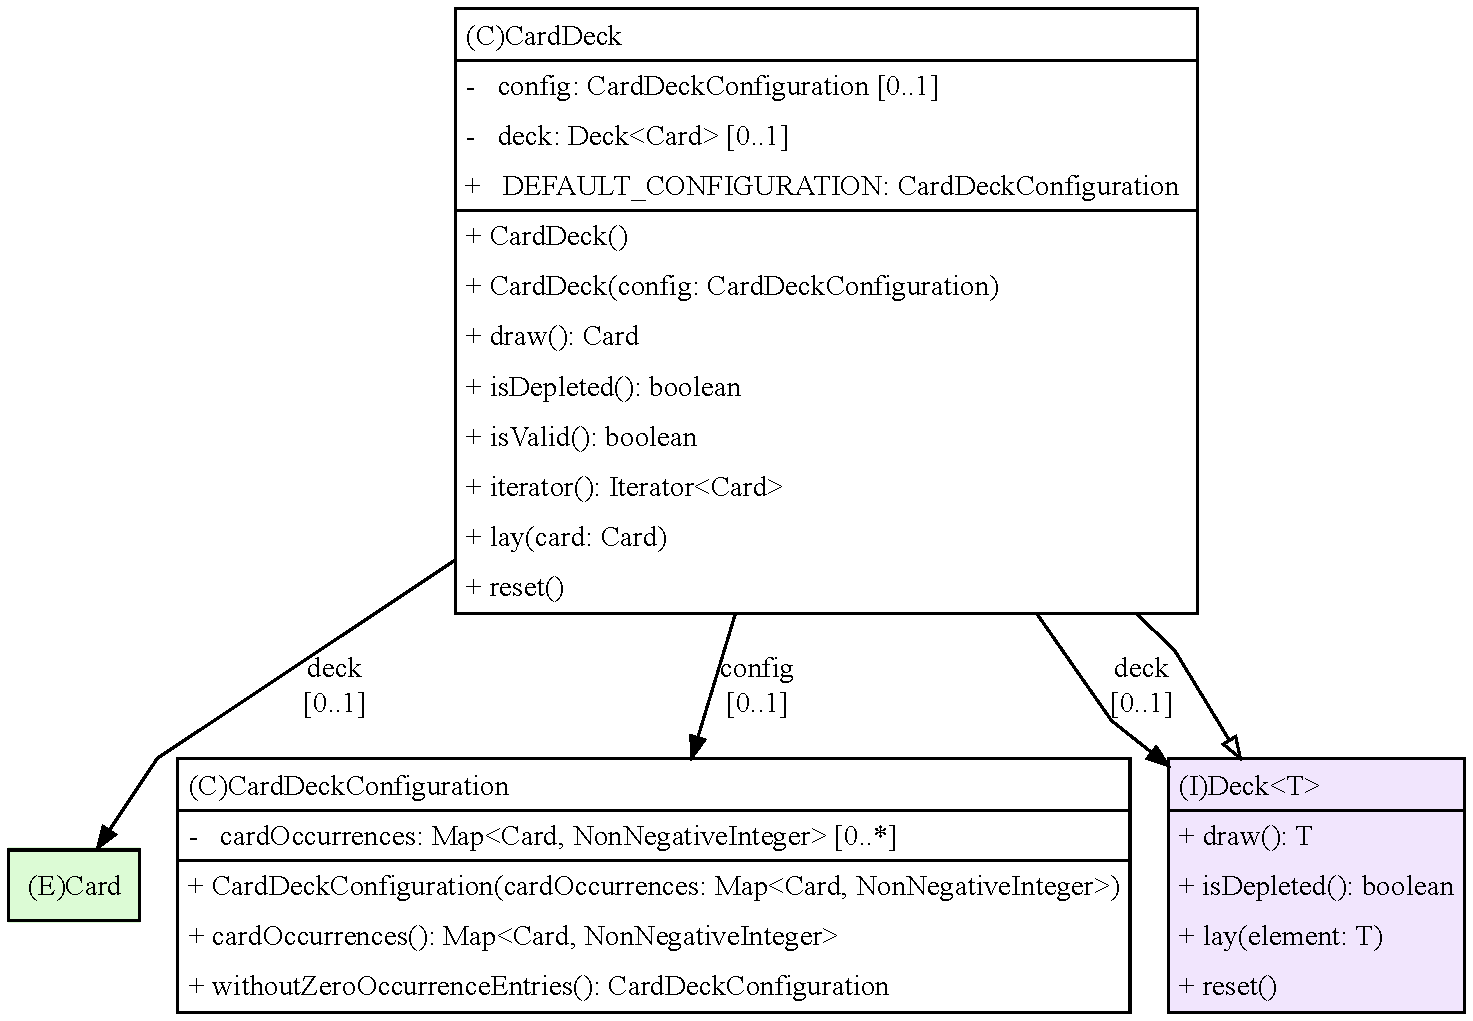
\includegraphics[width=0.85\textwidth]{Bilder/CardDeck_extract-before_structure.pdf} 
	\caption{UML-Diagramm von \textit{CardDeck} \underline{vor} der Method-Extraction.}
	\label{fig:extract-before}
\end{figure} 

\lstinputlisting[
	label=code:extract-method-after,    % Label; genutzt für Referenzen auf dieses Code-Beispiel
	caption=\underline{Nach} Method-Extraction der Methode \textit{countCardOccurrences} aus der \textit{isValid}-Methode in Commit \texttt{cb55ad97}.,
	captionpos=b,               % Position, an der die Caption angezeigt wird t(op) oder b(ottom)
	style=EigenerJavaStyle,   % Eigener Style der vor dem Dokument festgelegt wurde
	firstline=1,                % Zeilennummer im Dokument welche als erste angezeigt wird
	lastline=100                 % Letzte Zeile welche ins LaTeX Dokument übernommen wird
]{Quellcode/extract-method-after.java}

\begin{figure}[H]
	\centering
	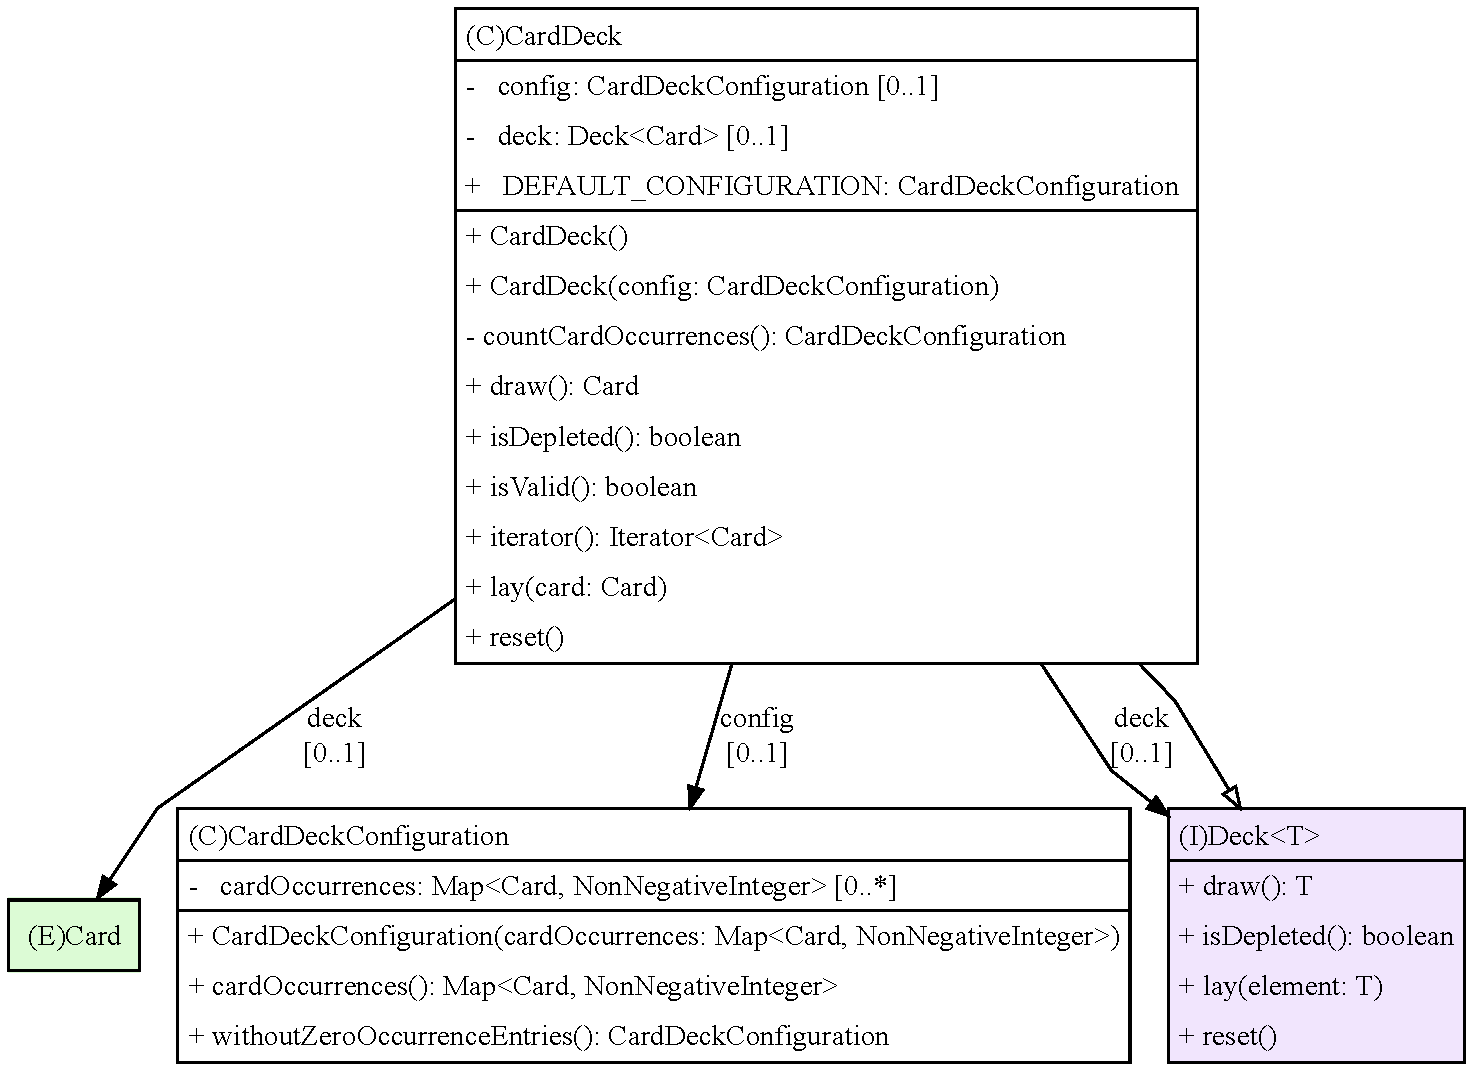
\includegraphics[width=0.85\textwidth]{Bilder/CardDeck_extract-after_structure.pdf} 
	\caption{UML-Diagramm von \textit{CardDeck} \underline{nach} der Method-Extraction durch Commit \texttt{cb55ad97}. 
	Beachte die neue private Methode \textit{countCardOccurrences} in \textit{CardDeck}.}
	\label{fig:extract-after}
\end{figure} 



\subsubsection{Replace-Temp-with-Query (RTQ)}

\autoref{fig:rtq-before} und \autoref{code:rtq-before} zeigen die \textit{execute}-Methode 
der \textit{StartCommand}-Klasse
\underline{vor} dem \textit{Replace-Temp-with-Query-(RTQ)}-Refactoring und \autoref{fig:rtq-after} und \autoref{code:rtq-after} \underline{nach}
dem Refactoring durch \underline{Commit \texttt{827cd843}}. \\
Das Extrahieren der Berechnung des \textit{CardDeck} von der \textit{execute}-Methode in die \textit{deckFrom}-Methode 
hilft dabei, dass die execute-Methode das SRP einhält und nur noch zuständig ist, den Output der \textit{start}-Methode 
der \textit{Game}-Klasse an den User auszugeben. Außerdem wird dadurch der \textit{Long-Method}-Code-Smell der 
\textit{execute}-Methode beseitigt.

\lstinputlisting[
	label=code:rtq-before,    % Label; genutzt für Referenzen auf dieses Code-Beispiel
	caption=\textit{execute}-Methode \underline{vor} RTQ-Refactoring.,
	captionpos=b,               % Position, an der die Caption angezeigt wird t(op) oder b(ottom)
	style=EigenerJavaStyle,   % Eigener Style der vor dem Dokument festgelegt wurde
	firstline=1,                % Zeilennummer im Dokument welche als erste angezeigt wird
	lastline=100                 % Letzte Zeile welche ins LaTeX Dokument übernommen wird
]{Quellcode/query-before.java}

\begin{figure}[H]
	\centering
	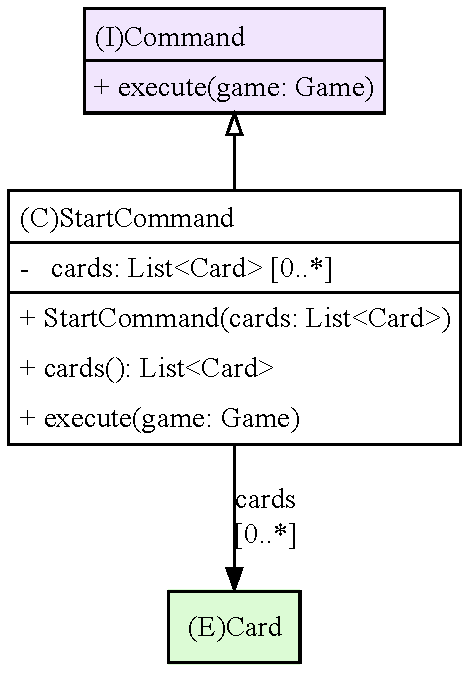
\includegraphics[width=0.4\textwidth]{Bilder/StartCommand_before_structure.pdf} 
	\caption{UML-Diagramm von \textit{StartCommand} \underline{vor} dem RTQ-Refactoring.}
	\label{fig:rtq-before}
\end{figure} 

\lstinputlisting[
	label=code:rtq-after,    % Label; genutzt für Referenzen auf dieses Code-Beispiel
	caption=\textit{execute}-Methode und \textit{deckFrom}-Methode \underline{nach} RTQ-Refactoring in Commit \texttt{827cd843}.,
	captionpos=b,               % Position, an der die Caption angezeigt wird t(op) oder b(ottom)
	style=EigenerJavaStyle,   % Eigener Style der vor dem Dokument festgelegt wurde
	firstline=1,                % Zeilennummer im Dokument welche als erste angezeigt wird
	lastline=100                 % Letzte Zeile welche ins LaTeX Dokument übernommen wird
]{Quellcode/query-after.java}

\begin{figure}[H]
	\centering
	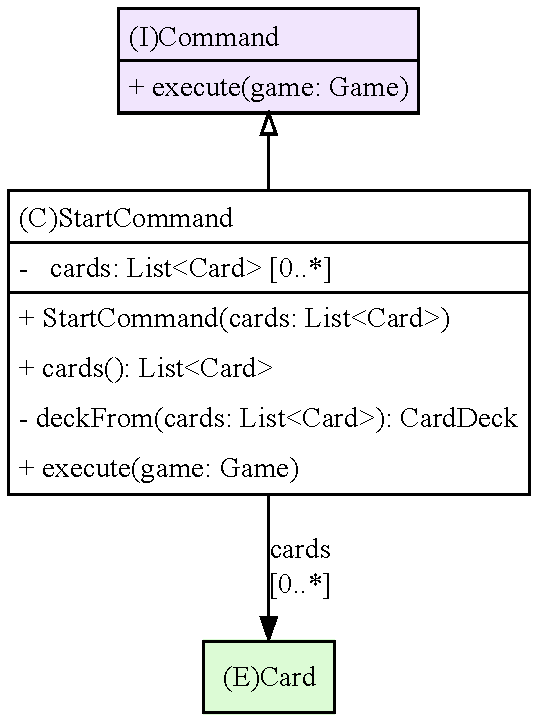
\includegraphics[width=0.4\textwidth]{Bilder/StartCommand_after_structure.pdf} 
	\caption{UML-Diagramm von \textit{StartCommand} \underline{nach} dem RTQ-Refactoring 
	durch Extraktion des Erstellens eines neuen Decks in Commit \texttt{827cd843}. 
	Beachte die neue private Methode \textit{countCardOccurrences} in \textit{CardDeck}.}
	\label{fig:rtq-after}
\end{figure} 